\section*{Microwave transitions in double-resonance trapped ions}

\begin{frame}{Working principle}

    The working principle is very similar to the one of the laser-cooled alkali metals, but with the \textbf{use of ions instead of atoms and a different cooling mechanism}.

    \begin{figure}
        \centering
        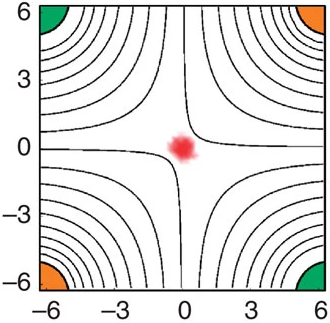
\includegraphics[height=0.35\textheight]{img/Paul-trapping-1.png}
        \hfill
        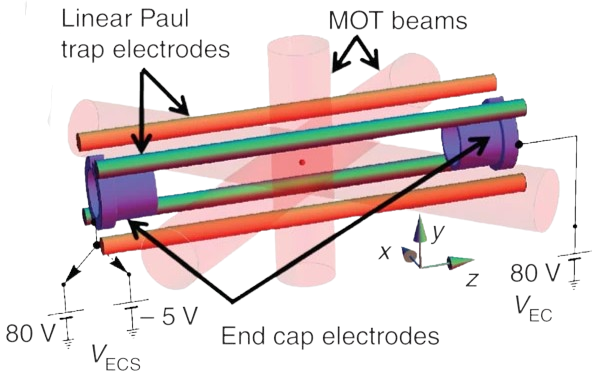
\includegraphics[height=0.35\textheight]{img/Paul-trapping-2.png}
        \caption{Schematic of the ion trapping setup (Paul trap).}
    \end{figure}

    The strong reduction of the Doppler broadening and the possibility of miniaturization makes this approach the most favorable for the NG-CSACs.

    \footnotetext[1]{MOT: Magneto-Optical Trap}

\end{frame}



\begin{frame}{Ytterbium based clock}

    \begin{columns}[c, onlytextwidth]

        \begin{column}{0.31\textwidth}

            \begin{figure}
                \centering
                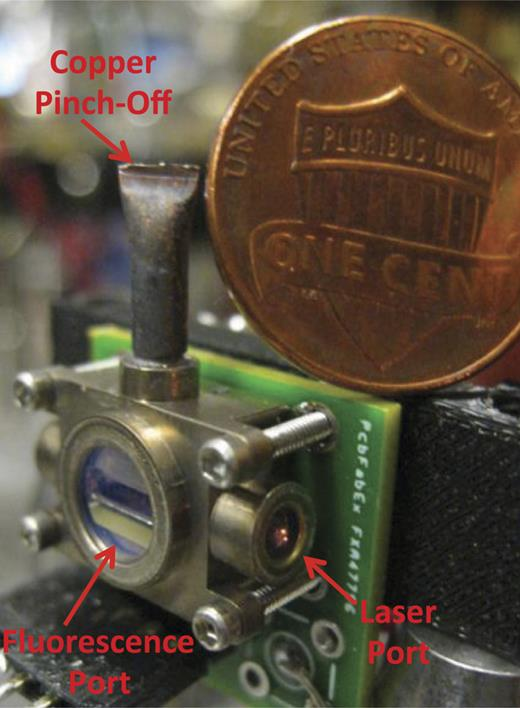
\includegraphics[width=\textwidth]{img/Ytterbium-clock.jpeg}
                \caption{Ion trap and vacuum package ($\approx 0.8cm^3$).}
            \end{figure}

        \end{column}

        \hfill

        \begin{column}{0.65\textwidth}

            One example of this technology is the $^{171}Yb^+$-based clock, \textbf{developed by Sandia and JPL (2015)}.

            \vspace{10pt}

            Known challenges and complications to achieve higher performances are:

            \begin{itemize}
                \item Stark Shift effect\footnotemark[1]: pulsed laser interrogation is required to avoid a shift in the ions transition frequency.
                \item Long life state $^2F_{7/2}$: the ions can fall into a long life state, from which must be released used an additional laser source or buffer gas.
            \end{itemize}

        \end{column}

    \end{columns}

    \footnotetext[1]{Start Shift effect: dependence of the atomic energy levels on the applied electric field.}

\end{frame}



\begin{frame}{Mercury based clock}

    Another example is the $^{199}Hg^+$-based clock, \textbf{developed by JPL (2019)} as a miniaturization of the current Deep Space Atomic Clock (DSAC).

    \vspace{10pt}

    \begin{columns}[c, onlytextwidth]

        \begin{column}{0.4\textwidth}

            \begin{figure}
                \centering
                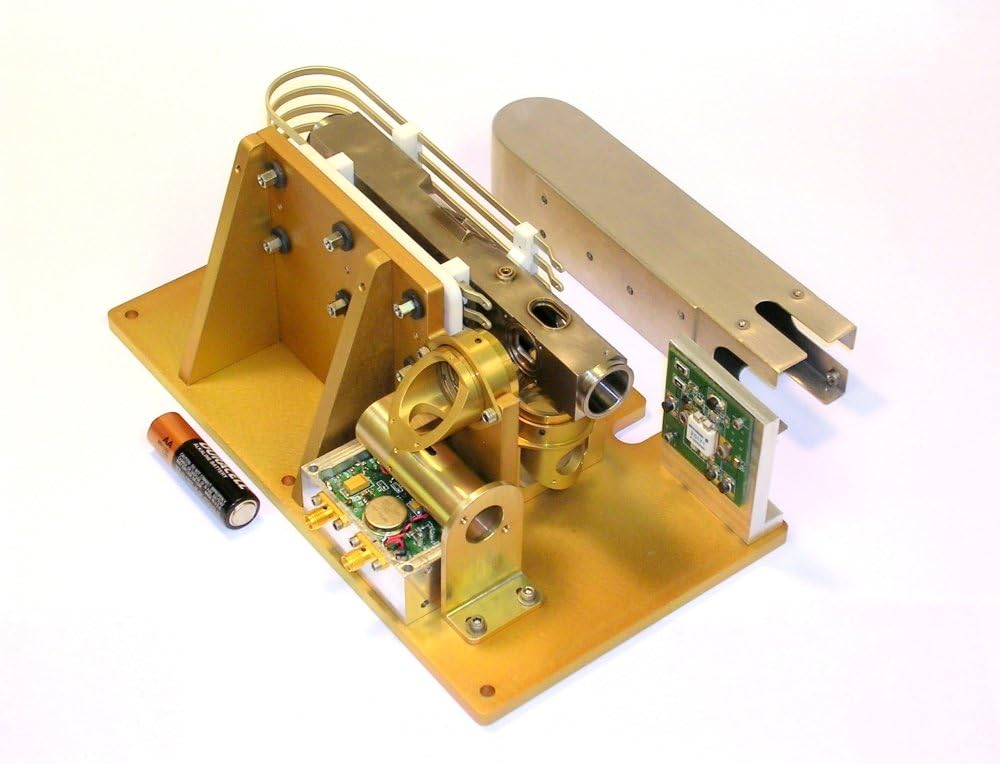
\includegraphics[width=0.9\textwidth]{img/Mercury-clock.jpg}
                \caption{Physics package ($\approx 3dm^3$).}
            \end{figure}

        \end{column}

        \hfill

        \begin{column}{0.55\textwidth}

            Born as a demonstration of the feasibility for a miniaturized version of the current DSAC with enhanced performances.

            \vspace{10pt}

            Its technology can be well suited adopted for a miniaturized version (NG-CSAC).

        \end{column}

    \end{columns}

\end{frame}



\begin{frame}{Current results}

    \begin{columns}[c, onlytextwidth]

        \begin{column}{0.5\textwidth}

            \begin{figure}
                \centering
                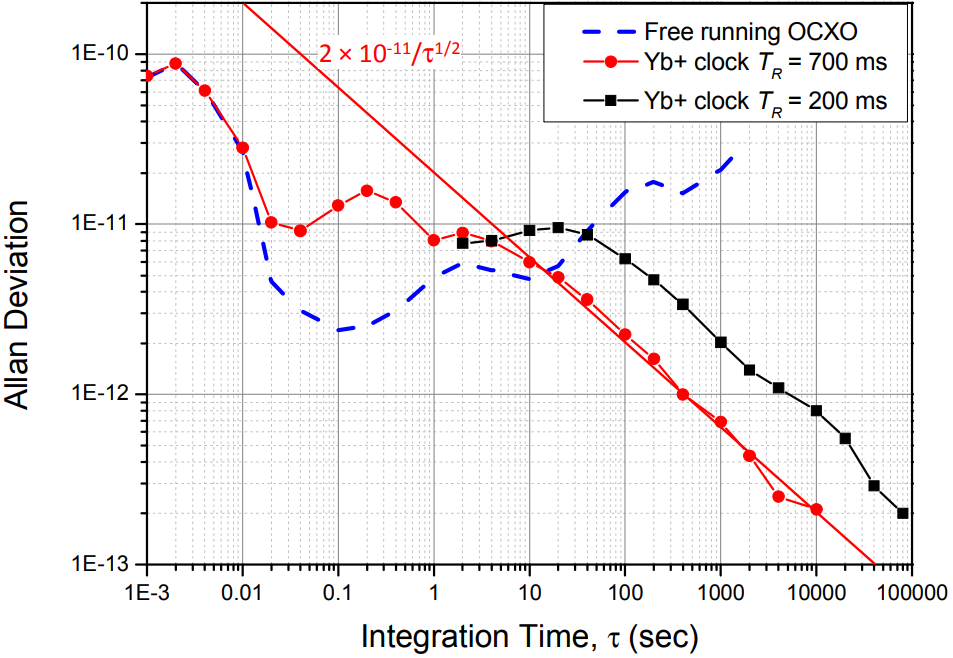
\includegraphics[height=0.4\textheight]{img/Ytterbium-stability.png}
                \caption{Sandia clock performances\footnotemark[1].}
            \end{figure}

        \end{column}

        \begin{column}{0.5\textwidth}

            \begin{figure}
                \centering
                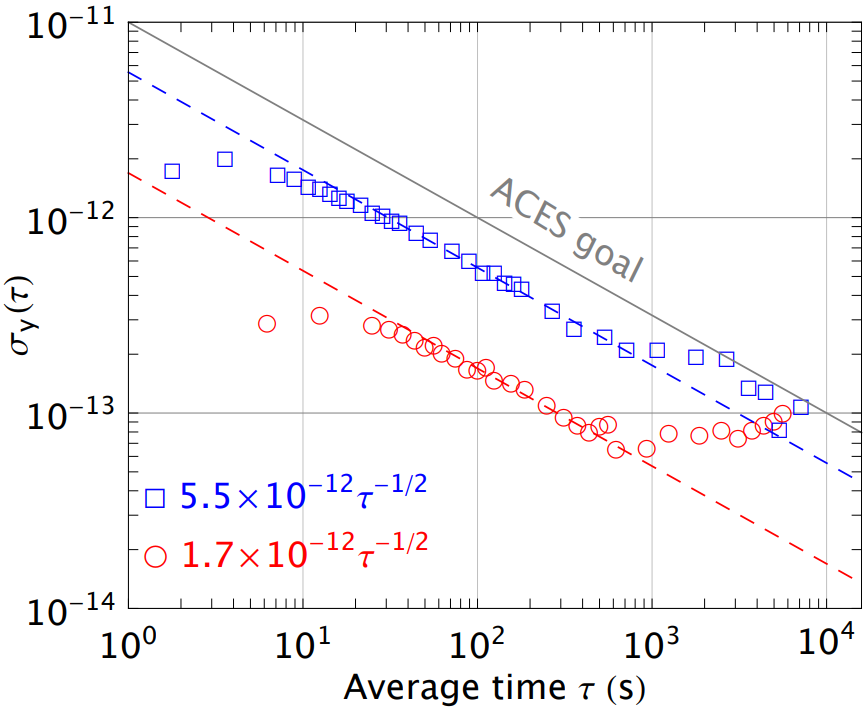
\includegraphics[height=0.4\textheight]{img/Mercury-stability.png}
                \caption{JPL clock performances\footnotemark[1].}
            \end{figure}

        \end{column}

    \end{columns}

    \vspace{10pt}

    \textbf{Trapped ions is probably the most promising solution for the NG-CSACs.}

    Further development is required to mitigate instabilities (Stark Shift effect) and reduce system complexity (pulsed laser interrogation).

    \footnotetext[1]{Performances are comparable recalling the different size of the two systems.}

\end{frame}